\section{C++中的 \lstinline|cin| 和 \lstinline|cout|}

\begin{frame}{\secname}
  \begin{itemize}
  \item  输入和输出并不是C++语言中的正式组成部分。
  \item C和C++本身都没有为输入和输出提供专门的语句结构。
  \item 输入输出不是由C++本身定义的,而是在编译系统提供的I/O库中定义的。
  \end{itemize}

\end{frame}

\begin{frame}{\secname}
  \begin{figure}[htbp]
    \centering
    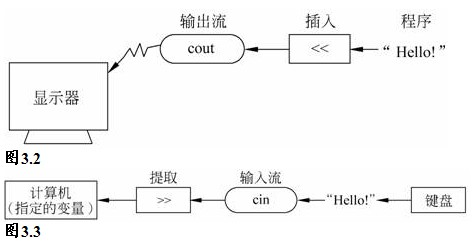
\includegraphics[width=4in]{slide04/images/cin_cout.jpg}
  \end{figure}
\end{frame}

\begin{frame}[fragile]{\secname}
  有关流对象\lstinline|cin|、\lstinline|cout|和流运算符的定义
  等信息是存放在C++的输入输出流库中的,因此如果在程序中使用\lstinline|cin|、\lstinline|cout|和流运算符,就必须使用预处理命令把头文件\lstinline|iostream|包含到本文件中:
  \begin{lstlisting}
#include <iostream>    
  \end{lstlisting}
\end{frame}

\begin{frame}[fragile]{\secname}
  \begin{itemize}
  \item \lstinline|cout| 语句的一般格式为
    \begin{lstlisting}
cout << expr1 << expr2 << ... << exprn;      
    \end{lstlisting}
  \item \lstinline|cin| 语句的一般格式为
    \begin{lstlisting}
cout >> var1 << var2 << ... << varn;      
    \end{lstlisting}
  \end{itemize} \pause 

  \begin{itemize}
  \item   在定义流对象时,系统会在内存中开辟一段缓冲区,用来暂存输入输出流的数据。


  \item 在执行\lstinline|cout|语句时,先把插入的数据顺序存放在输出缓冲区中,
  直到输出缓冲区满或遇到\lstinline|cout|语句中的\lstinline|endl|
  (或\lstinline|'\n'|)为止,此时将缓冲区中已有的数据一起输出,并清空缓冲区。

  \item 输出流中的数据在系统默认的设备(一般为显示器)输出。

  \end{itemize}
\end{frame}

\begin{frame}[fragile]{\secname}
  \begin{lstlisting}
cout << "This is a simple C++ program." << endl;    
\end{lstlisting}\pause
\begin{lstlisting}
cout << "This is "
     << "a simple C++ "
     << "program."
     << endl;    
  \end{lstlisting}\pause
\begin{lstlisting}
cout << "This is ";
cout << "a simple C++ ";
cout << "program.";
cout << endl;    
  \end{lstlisting}
\end{frame}

\begin{frame}[fragile]{\secname}
  \begin{free}[注]{}
    \begin{itemize}
    \item 不能用一个插入运算符 \lstinline|<<| 插入多个输出项,如:
      \begin{lstlisting}
cout << a, b, c; // wrong
cout << a+b+c;   // right, because a+b+c is an expression        
      \end{lstlisting}

    \item 在用\lstinline|cout|输出时,用户不必通知计算机按何种类型输出,
      系统会自动判别输出数据的类型,使输出的数据按相应的类型输出。
      如已定义\lstinline|a|为\lstinline|int|型,
      \lstinline|b|为\lstinline|float|型,
      \lstinline|c|为\lstinline|char|型,则
      \begin{lstlisting}
cout << a << ' ' << b << ' ' << c << endl;        
      \end{lstlisting}
      会以下面的形式输出:
      \begin{lstlisting}
4 345.789 a        
      \end{lstlisting}
    \end{itemize}
  \end{free}
\end{frame}

\begin{frame}[fragile]{\secname}
  \begin{lstlisting}
cin >> a >> b >> c >> d;    
  \end{lstlisting}\pause
  \begin{lstlisting}
cin >> a
    >> b
    >> c
    >> d;        
  \end{lstlisting}\pause
  \begin{lstlisting}
cin >> a;
cin >> b;
cin >> c;
cin >> d;    
\end{lstlisting}
以上三种情况可按如下形式从键盘输入:
\begin{lstlisting}
1 2 3 4[enter]  
\end{lstlisting}
\begin{lstlisting}
1[enter]
2 3[enter]
4[enter]  
\end{lstlisting}
\end{frame}

\begin{frame}[fragile]{\secname}
  \begin{free}[注]{}
    在用\lstinline|cin|输入时,系统也会根据变量的类型从输入流中提取相应长度的字节。
    如
    \begin{lstlisting}
char c1, c2;
int a;
float b;
\end{lstlisting}
若输入
\begin{lstlisting}
1234 56.78  
\end{lstlisting}
则\lstinline|c1, c2, a, b|分别被赋值为\lstinline|'1', '2', 34, 56.78|。
  \end{free}
\end{frame}


\begin{frame}[fragile]{控制符的使用}
  上面介绍的是使用\lstinline|cout|和\lstinline|cin|时的默认格式。
  但有时人们在输入输出时有一些特殊的要求,
  如在输出实数时规定字段宽度,只保留两位小数,数据向左或向右对齐等。
  C++提供了在输入输出流中使用的控制符。

  需要注意的是: \red{如果使用了控制符,
    在程序开头除了要加\lstinline|iostream|头文件外,
    还要加\lstinline|iomanip|头文件。}
\end{frame}